\documentclass[crop, tikz]{standalone}

\usepackage[utf8]{inputenc}
% 'crop' is the default for v1.0, before it was 'preview'
%\usetikzlibrary{...}% tikz package already loaded by 'tikz' option

\usetikzlibrary{arrows}
\usetikzlibrary{decorations.markings}

\begin{document}

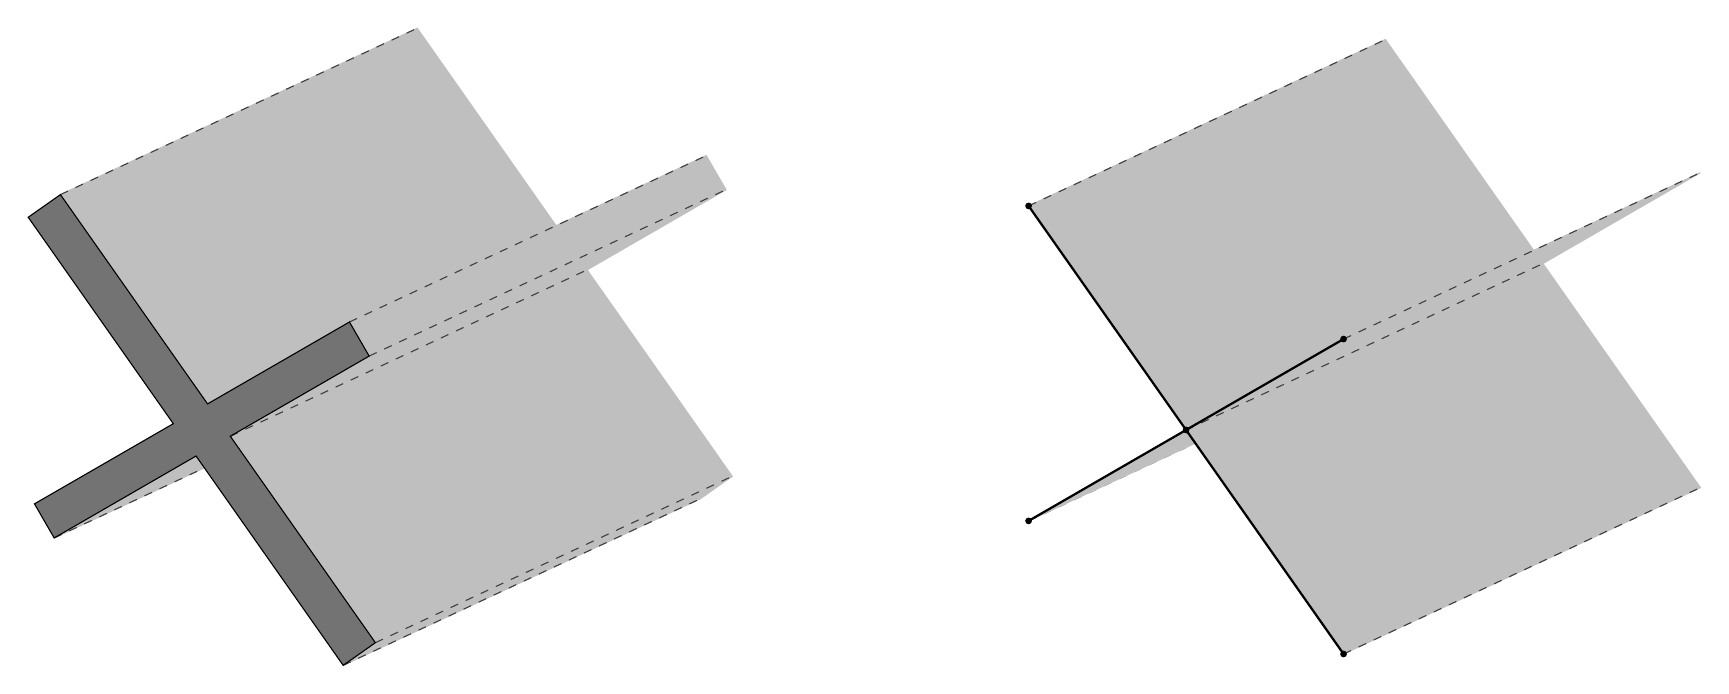
\begin{tikzpicture}

	%Graph in the 2D plane, place on the right ideally.
	\pgfdeclarelayer{foreground}
	\pgfdeclarelayer{background}
	\pgfsetlayers{background,main,foreground}

	%declare constants
	\def\ang{65}
	\def\extAng{25}
	\def\mag{2.0}
	\def\extLeng{5.0}

	%extruded graph
	\begin{scope}[shift={(12.5,0)}]
		\coordinate (centre) at (0,0);
		\coordinate (vNW) at ({-\mag},{\mag * (1+cos(\ang))});
		\coordinate (vNE) at ({\mag},{\mag * (1-cos(\ang))});
		\coordinate (vSE) at ({\mag},{-\mag * (1+cos(\ang))});
		\coordinate (vSW) at ({-\mag},{-\mag * (1-cos(\ang))});
		\coordinate (centrePlaneEnd) at ({\extLeng * cos(\extAng)}, {\extLeng*sin(\extAng)});
		\coordinate (vNWPlaneEnd) at ({-\mag + \extLeng * cos(\extAng)},{\mag * (1+cos(\ang)) + \extLeng*sin(\extAng)});
		\coordinate (vNEPlaneEnd) at ({\mag + \extLeng * cos(\extAng)},{\mag * (1-cos(\ang)) + \extLeng*sin(\extAng)});
		\coordinate (vSEPlaneEnd) at ({\mag + \extLeng * cos(\extAng)},{-\mag * (1+cos(\ang)) + \extLeng*sin(\extAng)});
		\coordinate (vSWPlaneEnd) at ({-\mag + \extLeng * cos(\extAng)},{-\mag * (1-cos(\ang)) + \extLeng*sin(\extAng)});
		\begin{pgfonlayer}{foreground}
			%graph edges
			\draw[thick] (centre) -- (vNW);
			\draw[thick] (centre) -- (vNE);
			\draw[thick] (centre) -- (vSE);
			\draw[thick] (centre) -- (vSW);
			%graph vertices
			\filldraw[black] (centre) circle (1pt);
			\filldraw[black] (vNW) circle (1pt);
			\filldraw[black] (vNE) circle (1pt);
			\filldraw[black] (vSE) circle (1pt);
			\filldraw[black] (vSW) circle (1pt);
		\end{pgfonlayer}
		%extruded planes, draw planes coming out at an angle of \extAng degrees, with length 5
		%plane outlines
		\draw[dashed, black!75!white] (centre) -- (centrePlaneEnd);
		\draw[dashed, black!75!white] (vNW) -- (vNWPlaneEnd);
		\draw[dashed, black!75!white] (vNE) -- (vNEPlaneEnd);
		\draw[dashed, black!75!white] (vSE) -- (vSEPlaneEnd);
		\begin{pgfonlayer}{background}
			\draw[dashed, black!75!white] (vSW) -- (vSWPlaneEnd);
		\end{pgfonlayer}
		%plane fills
		\begin{pgfonlayer}{background}
			\filldraw[black!25!white] (vNW) -- (vNWPlaneEnd) -- (centrePlaneEnd) -- (centre) -- cycle;
			\filldraw[black!25!white] (vNE) -- (vNEPlaneEnd) -- (centrePlaneEnd) -- (centre) -- cycle;
			\filldraw[black!25!white] (vSE) -- (vSEPlaneEnd) -- (centrePlaneEnd) -- (centre) -- cycle;
			\filldraw[black!25!white] (vSW) -- (vSWPlaneEnd) -- (centrePlaneEnd) -- (centre) -- cycle;
		\end{pgfonlayer}
	\end{scope}

	%extruded thin structure
	%the width of the thin-structure will be 0.25 (default Tikz unit), although we may want this labelled at a later date.
	%we will inherit the extrusion properties of the graph-portion of the diagram.
	%use the DiagramPointFinding.py script to compute these values!
	\begin{scope}[shift={(0,0)}]
		\coordinate (vNWbl) at (-2.204526124401337, +2.701469126491091);
		\coordinate (vNWtr) at (-1.7954738755986637, +2.9890039204717067);
		\coordinate (vNInt) at (0.07302546412888766, +0.330842637724853);
		\coordinate (vNEtl) at (1.8749948901643632, +1.37126687721933);
		\coordinate (vNEbr) at (2.125005109835637, +0.9382600758178719);
		\coordinate (vEInt) at (0.361704532437812, -0.07983747663371243);
		\coordinate (vSEtr) at (2.204526124401337, -2.7014691264910913);
		\coordinate (vSEbl) at (1.7954738755986628, -2.9890039204717076);
		\coordinate (vSInt) at (-0.07302546412888922, -0.330842637724853);
		\coordinate (vSWbr) at (-1.8749948901643634, -1.3712668772193293);
		\coordinate (vSWtl) at (-2.125005109835637, -0.9382600758178719);
		\coordinate (vWInt) at (-0.3617045324378124, +0.07983747663371221);
		\begin{pgfonlayer}{foreground}
			%2D-structure border
			\filldraw[black!55!white, draw=black] (vNWbl) -- (vNWtr) -- (vNInt) -- (vNEtl) -- (vNEbr) -- (vEInt) -- (vSEtr) -- (vSEbl) -- (vSInt) -- (vSWbr) -- (vSWtl) -- (vWInt) -- cycle;
		\end{pgfonlayer}
		%extruded planes, draw planes coming out at an angle of 25 degrees, with length 5
		%coordinates for plane endpoints
		\coordinate (originEX) at (4.531538935183249, +2.1130913087034973);
		\coordinate (vNWtrEX) at (2.7360650595845857, +5.1020952291752035);
		\coordinate (vNWblEX) at (2.327012810781912, +4.814560435194588);
		\coordinate (vNEbrEX) at (6.656544045018887, +3.051351384521369);
		\coordinate (vNEtlEX) at (6.406533825347612, +3.484358185922827);
		\coordinate (vSEblEX) at (6.327012810781913, -0.8759126117682103);
		\coordinate (vSEtrEX) at (6.736065059584586, -0.588377817787594);
		\coordinate (vSWtlEX) at (2.4065338253476125, +1.1748312328856254);
		\coordinate (vSWbrEX) at (2.6565440450188857, +0.741824431484168);
		\coordinate (vNIntEX) at (4.604564399312137, +2.4439339464283503);
		\coordinate (vEIntEX) at (4.893243467621061, +2.033253832069785);
		\coordinate (vSIntEX) at (4.45851347105436, +1.7822486709786443);
		\coordinate (vWIntEX) at (4.169834402745437, +2.1929287853372097);
		%plane outlines, only need the ones which will still be visible after overlay
		\draw[dashed, black!75!white] (vNWtr) -- (vNWtrEX);
		\draw[dashed, black!75!white] (vNEbr) -- (vNEbrEX);
		\draw[dashed, black!75!white] (vNEtl) -- (vNEtlEX);
		\draw[dashed, black!75!white] (vEInt) -- (vEIntEX);
		\draw[dashed, black!75!white] (vSEbl) -- (vSEblEX);
		\draw[dashed, black!75!white] (vSEtr) -- (vSEtrEX);
		\begin{pgfonlayer}{background}
			%plane fills
			\filldraw[black!25!white] (vSWbr) -- (vSWbrEX) -- (vSIntEX) -- (vSInt) -- cycle;
			\draw[dashed, black!75!white] (vSWbr) -- (vSWbrEX);
			\filldraw[black!25!white] (vNWtr) -- (vNWtrEX) -- (vNIntEX) -- (vNInt) -- cycle;
			\filldraw[black!25!white] (vNEtl) -- (vNEtlEX) -- (vNEbrEX) -- (vNEbr) -- cycle;
			\filldraw[black!25!white] (vNEbr) -- (vNEbrEX) -- (vEIntEX) -- (vEInt) -- cycle;
			\filldraw[black!25!white] (vEInt) -- (vEIntEX) -- (vSEtrEX) -- (vSEtr) -- cycle;
			\filldraw[black!25!white] (vSEtr) -- (vSEtrEX) -- (vSEblEX) -- (vSEbl) -- cycle;
		\end{pgfonlayer}
	\end{scope}

\end{tikzpicture}

\end{document}